\section{Materials}\label{sec:materials}

\subsection{Data}\label{sec:data}

The multi-parametric \ac{mri} data are acquired from a cohort of patients with higher-than-normal level of \ac{psa}.
The acquisition is performed using a 3T whole body \ac{mri} scanner (Siemens Magnetom Trio TIM, Erlangen, Germany) using sequences to obtain \ac{t2w}-\ac{mri}, \ac{dce}-\ac{mri} and \ac{dw}-\ac{mri}.
Aside of the \ac{mri} examination, these patients also have undergone a guided-biopsy.
The dataset is composed of a total of 20 patients of which 18 patients have biopsy proven \ac{cap} and 2 patients are ``healthy'' with negative biopsies.
Therefore, 13 patients have a \ac{cap} in the \ac{pz}, 3 patients have \ac{cap} in the \ac{cg}, 2 patients have invasive \ac{cap} in both \ac{pz} and \ac{cg} and finally 2 patients are considered as ``healthy''.
An experienced radiologist has segmented the prostate organ --- on \ac{t2w}-\ac{mri} and \ac{dce}-\ac{mri} --- as well as the prostate zones (i.e., \ac{pz} and \ac{cg}) and \ac{cap} on the \ac{t2w}-\ac{mri}.

A \SI{3}{\mm} slice fat-suppressed \ac{t2w} fast spin-echo sequence (\ac{tr}/\ac{te}/\ac{etl}: \SI{3400}{\ms}/\SI{85}{\ms}/13) is used to acquire images in sagittal and oblique coronal planes, the latter planes being orientated perpendicular or parallel to the prostate \ac{pz} – rectal wall axis.
Three-dimensional \ac{t2w} fast spin-echo (\ac{tr}/\ac{te}/\ac{etl}: \SI{3600}{\ms}/\SI{143}{\ms}/109, slice thickness: \SI{1.25}{\mm}) images are then acquired in an oblique axial plane.
The nominal matrix and \ac{fov} of the 3D \ac{t2w} fast spin-echo images are $320 \times 256$ and $280 \times 240$ mm\textsuperscript{2}, respectively, thereby affording sub-millimetric pixel resolution within the imaging plane.

\ac{dce}-\ac{mri} is performed using a fat suppressed 3D T$_1$ VIBE sequence (\ac{tr}/\ac{te}/Flip angle: \SI{3.25}{\ms}/\SI{1.12}{\ms}/\SI{10}{\degree}; Matrix: $256 \times 192$; \ac{fov}: $280 \times 210$ (with 75\% rectangular \ac{fov}); slab of 16 partitions of \SI{3.5}{\mm} thickness; temporal resolution: \SI{6}{\s}/slab over approximately \SI{5}{\minute}).
A power injector (Medrad, Indianola, USA) is used to provide a bolus injection of Gd-DTPA (Dotarem, Guerbet, Roissy, France) at a dose of \SI{0.2}{\ml} Gd-DTPA/kg of body weight.

These \ac{dce}-\ac{mri} sequences are resampled using the spatial information of the \ac{t2w}-\ac{mri} and missing data are interpolated using a linear interpolation.
The volumes of the \ac{dce}-\ac{mri} dynamic are rigidly registered, to remove any patient motion during the acquisition.
Furthermore, a non-rigid registration is performed between the \ac{t2w}-\ac{mri} and \ac{dce}-\ac{mri} in order to propagate the prostate zones and \ac{cap} ground-truths.
The resampling is implemented in C++ using the Insight Segmentation and Registration Toolkit~\citep{ibanez2005itk}.

\subsection{Implementation}

The implementation of the registration (C++), normalization (Python), and classification pipeline (Python) are publicly available on GitHub\footnote{\url{https://github.com/I2Cvb/lemaitre-2016-nov/tree/master}}~\citep{lemaitre2016github}.
The data used for this work are also publicly available\footnote{\url{https://zenodo.org/record/61163}}~\citep{lemaitre2016dce}.

\section{Experiments and results}\label{sec:experiments}

\subsection{Goodness of model fitting}\label{sec:fit}

%{\color{red} In case that we have issue with $R^2$, we need to provide the AIC since that the model are usually non-linear.}

\begin{table*}
  \caption{Coefficient of determination $R^{2}$ (i.e., $\mu \ (\pm \sigma)$), while fitting data with the different quantification models.}
  \centering
  \resizebox{\columnwidth}{!}{
  \begin{tabular}{lc c c c c c}
    \toprule
    Data type & Brix & Hoffmann & Tofts population \ac{aif} & Tofts patient \ac{aif} & \ac{pun} & Semi-quantitative \\
    \midrule
    Un-normalized & $0.85 \ (\pm 0.11)$ & $0.81 \ (\pm 0.17)$ & $0.84 \ (\pm 0.14)$ & $0.88 \ (\pm 0.12)$ & $0.27 \ (\pm 0.18)$ & $0.64 \ (\pm 0.24)$  \\
    Normalized    & $0.92 \ (\pm 0.05)$ & $0.72 \ (\pm 0.32)$ & $0.92 \ (\pm 0.06)$ & $0.90 \ (\pm 0.10)$ & $0.28 \ (\pm 0.20)$ & $0.75 \ (\pm 0.20)$  \\
    \bottomrule
  \end{tabular}
  }
  \label{tab:r2}
\end{table*}

Parameter estimation of the quantification methods are related to fit a specific model to the \ac{dce}-\ac{mri} data.
Therefore, this section report the goodness of fitting by computing the coefficient of determination $R^2$ such as in Eq.\,\eqref{eq:r2}

\begin{equation}
  R^2 = 1 - \frac{\sum_{t = 1}^{T} (s_t - \hat{s}_t)^2}{\sum_{t = 1}^{T} (s_t - \bar{s})^2} ,
  \label{eq:r2}
\end{equation}

\noindent where $s_t$ and $\hat{s}_t$ are the signal to be fitted and the estimated signal at time $t$, respectively; $\bar{s}$ is the average signal to be fitted.

Mean and standard-deviation of the coefficient of determination $R^{2}$ is reported in Table~\ref{tab:r2} for each quantification model.
Brix, Hoffmann, and Tofts models are fitted with a coefficient $R^{2}$ superior to 0.80.
Additionally, the proposed \ac{pun} model does not seem to fit well the data.
Data normalization improves the coefficient $R^2$ for all the methods apart of the Hoffmann model.
The large standard deviation for this model might imply that there are some cases where the fitting fails.

\subsection{Detection of \acs*{cap} using pharmacokinetic parameters}

\begin{table*}
  \caption{\acs*{auc} (i.e., $\mu \ (\pm \sigma)$) for each individual pharmacokinetic parameter using a \acs*{rf} classifier.}
  \centering
  \resizebox{\columnwidth}{!}{
  \begin{tabular}{l c c}
    \toprule
    \textbf{Features} & Un-normalized data & Normalized data \\
    \midrule
    \textbf{Brix model} & & \\
    \quad $A$         & $0.540\ (\pm 0.069)$ & $0.555\ (\pm 0.080)$ \\
    \quad $k_{el}$    & $0.549\ (\pm 0.062)$ & $0.577\ (\pm 0.093)$ \\
    \quad $k_{ep}$    & $0.506\ (\pm 0.032)$ & $0.497\ (\pm 0.019)$ \\
    \textbf{Hoffmann model} & & \\
    \quad $A$         & $0.516\ (\pm 0.020)$ & $0.508\ (\pm 0.031)$ \\
    \quad $k_{el}$    & $0.545\ (\pm 0.066)$ & $0.529\ (\pm 0.065)$ \\
    \quad $k_{ep}$    & $0.550\ (\pm 0.063)$ & $0.545\ (\pm 0.060)$ \\
    \textbf{Tofts model with population \ac{aif}} & & \\
    \quad $K_{trans}$ & $0.556\ (\pm 0.086)$ & $0.565\ (\pm 0.097)$ \\
    \quad $k_{ep}$    & $0.506\ (\pm 0.026)$ & $0.528\ (\pm 0.038)$ \\
    \quad $v_{p}$     & $0.533\ (\pm 0.064)$ & $0.548\ (\pm 0.082)$ \\
    \textbf{Tofts model with patient \ac{aif}} & & \\
    \quad $K_{trans}$ & $0.563\ (\pm 0.077)$ & $0.548\ (\pm 0.060)$ \\
    \quad $k_{ep}$    & $0.492\ (\pm 0.025)$ & $0.491\ (\pm 0.020)$ \\
    \quad $v_{p}$     & $0.530\ (\pm 0.069)$ & $0.495\ (\pm 0.033)$ \\
    \textbf{\ac{pun} model} & & \\
    \quad $a_0$       & $0.521\ (\pm 0.040)$ & $0.530\ (\pm 0.045)$ \\
    \quad $r$         & $0.550\ (\pm 0.085)$ & $0.573\ (\pm 0.097)$ \\
    \quad $\beta$     & $0.531\ (\pm 0.051)$ & $0.549\ (\pm 0.068)$ \\
    \textbf{Semi-quantitative analysis} & & \\
    \quad wash-in     & $0.587\ (\pm 0.107)$ & $0.533\ (\pm 0.032)$ \\
    \quad wash-out    & $0.516\ (\pm 0.037)$ & $0.486\ (\pm 0.035)$ \\
    \quad IAUC        & $0.506\ (\pm 0.048)$ & $0.513\ (\pm 0.032)$ \\
    \quad $\tau$      & $0.565\ (\pm 0.104)$ & $0.537\ (\pm 0.089)$ \\
    \quad $S_M - S_0$ & $0.560\ (\pm 0.083)$ & $0.532\ (\pm 0.029)$ \\
    \bottomrule
  \end{tabular}
  }
  \label{tab:resfeats}
\end{table*}

\begin{figure*}
  \centering
  \hspace*{\fill}
  \subfigure[Without normalization.]{\label{fig:rfpharmaunorm}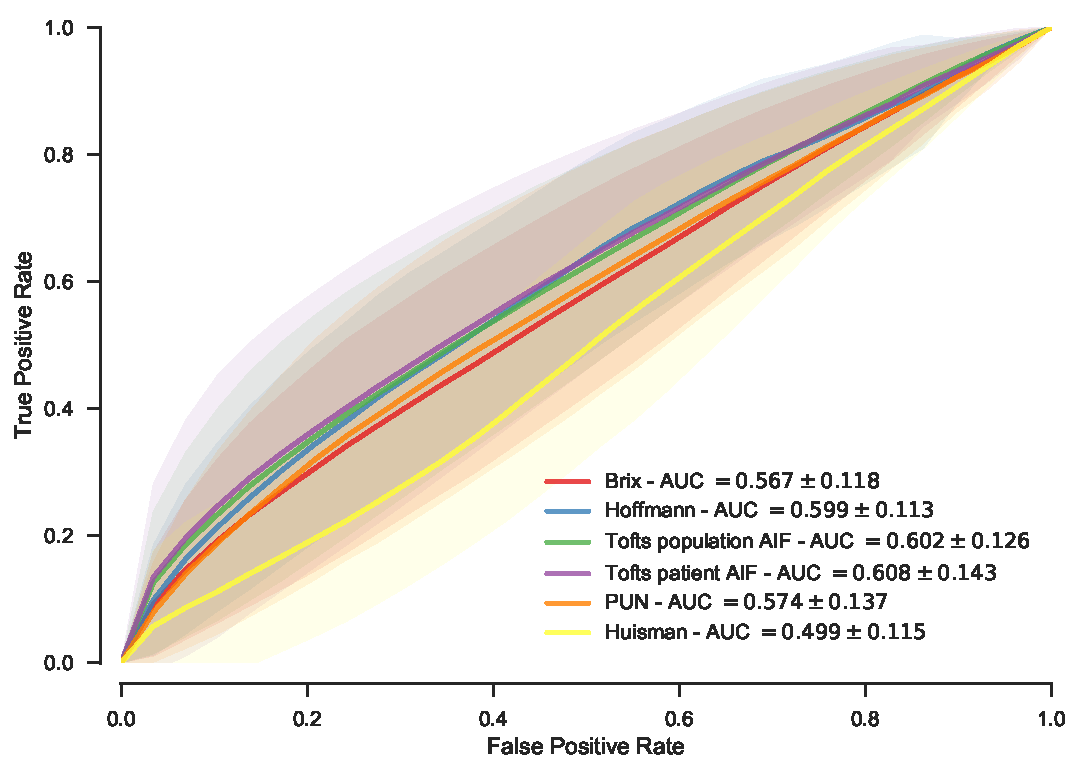
\includegraphics[width=.49\textwidth]{03_experiments/figures/unormalized/unormalized_methods_0.pdf}} \hfill
  \subfigure[With normalization.]{\label{fig:rfpharmanorm}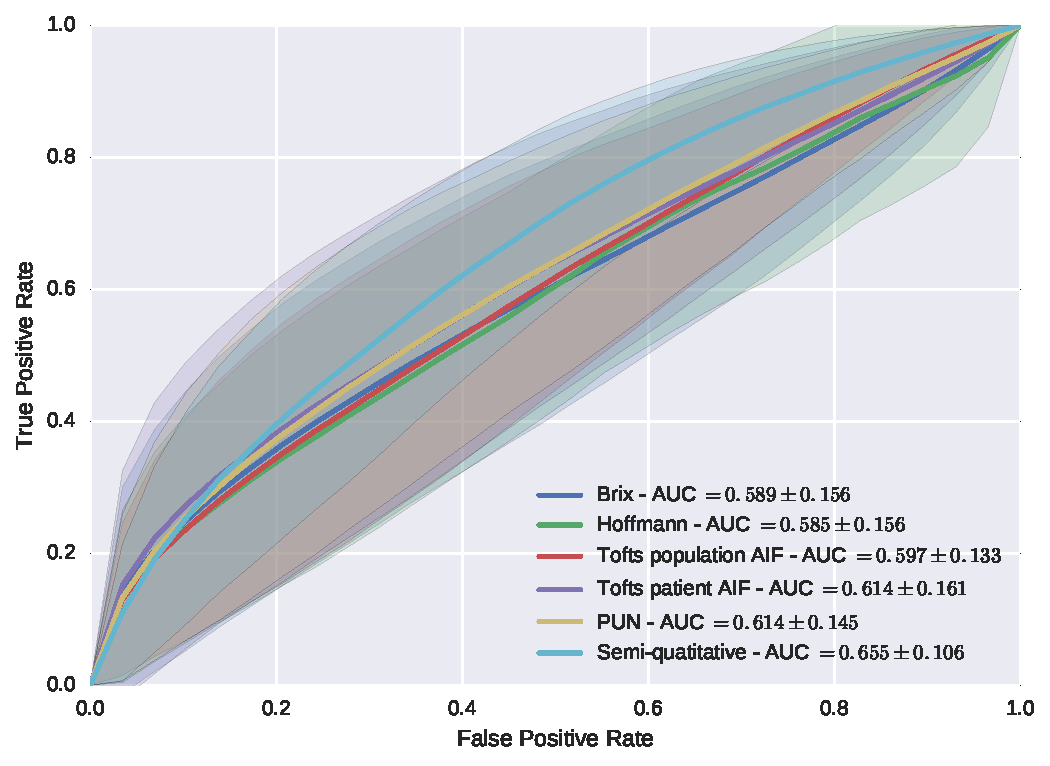
\includegraphics[width=.49\textwidth]{03_experiments/figures/normalized/normalized_methods_0.pdf}}
  \hspace*{\fill}
  \caption{\acs*{roc} analysis using a \acs*{rf} classifier with and without normalization \ac{dce}-\ac{mri} data for different pharmacokinetic models.}
  \label{fig:normpharmarf}
\end{figure*}

To study the potential benefit of our normalization, \ac{cap} are detected at a voxel level using pharmacokinetic parameters estimated from un-normalized and normalized \ac{dce}-\ac{mri} data.
Each individual pharmacokinetic parameter is classified to evaluate their individual discriminative power to detect \ac{cap}.
Therefore, a \ac{rf} classifier is used in conjunction with a \ac{lopo}.
The use of \ac{rf} is motivated since that it leads to the best performance in the state-of-the-art methods~\citep{litjens2014computer,lemaitre2015computer}.
Results are summarized in Table~\ref{tab:resfeats} in terms of \ac{auc}.
Normalization can improve the detection of \ac{cap}; however, the benefit of normalization is more obvious by combining together the pharmacokinetic features of a given model (e.g., $A$, $k_ep$, and $k_el$ for Brix model), as previously done in traditional \ac{cad} system~\citep{lemaitre2015computer}.
For the latter configuration, results are summarized by performing a \ac{roc} analysis and computing the \ac{auc}, as reported in Fig.\,\ref{fig:normpharmarf}.
Quantification using normalized data outperforms quantification using un-normalized data in terms of classification performance apart of Hoffmann and Tofts population-based \ac{aif} models.
The reasons behind the decrease of the \ac{auc} might be related to: (i) a poor fitting as discussed in Sect.\,\ref{sec:fit} (cf., Hoffmann model) and (ii) a small number of patients while estimating some parameters (cf., Tofts model).
The best classification performance are obtained using the semi-quantitative approach with an \ac{auc} of 0.655.

\subsection{Classification of the entire enhanced \acs*{dce}-\acs*{mri} signal}

\begin{figure}
  \centering
  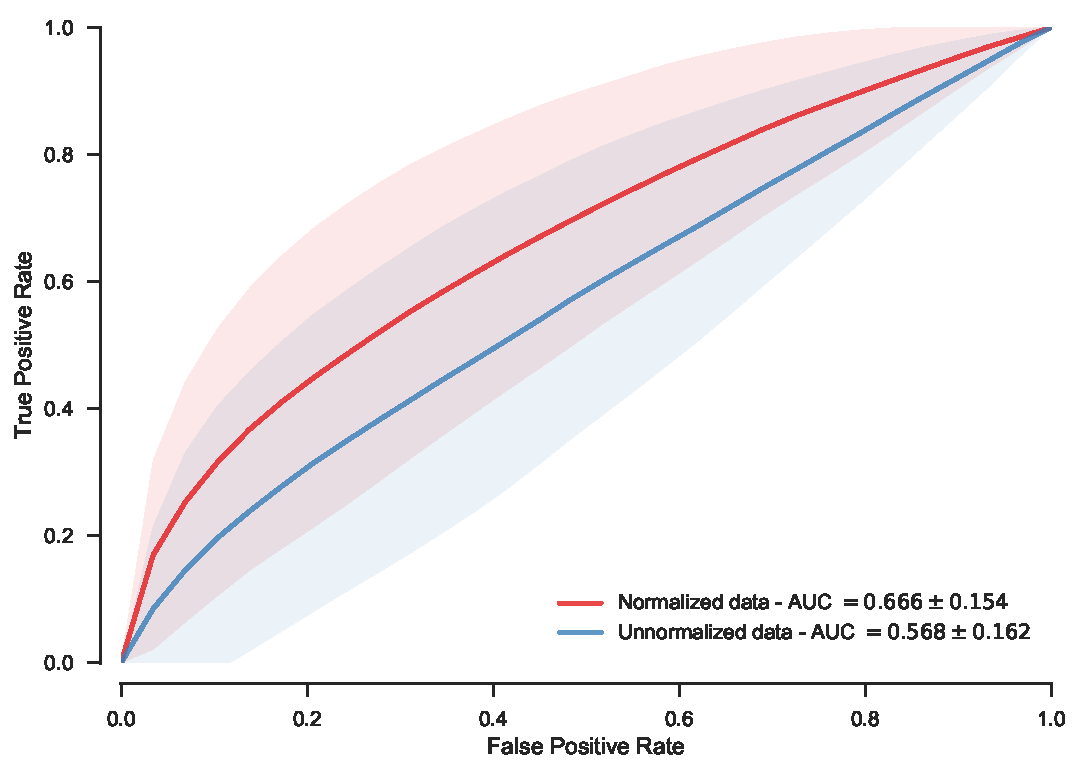
\includegraphics[width=0.7\linewidth]{03_experiments/figures/full_signal_0.pdf}
  \caption{\acs*{roc} analysis using the entire \ac{dce}-\ac{mri} signal with and without normalization in conjunction with a \acs*{rf} classifier.}
  \label{fig:rfnormdcesignal}
\end{figure}

As stated in the introduction, the quantification methods are extracting a set of parameters characterizing the enhancement \ac{dce}-\ac{mri} signal.
However, this extraction might lead to a loss of information.
This experiment is performed to assess if making use of the whole \ac{dce}-\ac{mri} signal instead of the just the pharmacokinetic parameters can improve the classification performance.
Therefore, each enhanced \ac{dce}-\ac{mri} signal, normalized and un-normalized, is classified using a \ac{rf} classifier in a \ac{lopo} fashion.
The \ac{roc} analysis and \ac{auc} are reported in Fig.\,\ref{fig:rfnormdcesignal}.
Classification without normalization lead to the worst performance, with an \ac{auc} of 0.568.
However, data normalization in conjunction with the use of the whole \ac{dce}-\ac{mri} signal is the strategy which outperforms all others, with an \ac{auc} of 0.666.

%%% Local Variables: 
%%% mode: latex
%%% TeX-master: "../main"
%%% End: 
